\documentclass[xcolor=dvipsnames]{beamer}

\usepackage[utf8x]{inputenc}
\usepackage{float}
\usepackage{graphicx}

\usetheme{Dresden}
\usecolortheme[named=Bittersweet]{beaver}

% \definecolor{darkgray}{RGB}{69, 69, 69}
% \setbeamercolor{normal text}{fg=darkgray}
\setbeamercolor{title}{bg=white}
\setbeamerfont{title}{size={\fontsize{56}{58}}}

\title{Dynamite!}
\author{Alexandru Fikl \and Adrian Breaz}
\date{December 1, 2011}

\begin{document}

\begin{frame}
 \titlepage
\end{frame}

\begin{frame}
 \frametitle{Today We're Gonna Talk About:}
 \tableofcontents
\end{frame}

\section{The History}
\begin{frame}{History}
\begin{itemize}
    \item Around 1860 Alfred Nobel started experimenting with nitroglycerin.
	\item Nitroglycerin was first invented by Italian chemist Ascanio Sobrero
in 1846.
	\item In 1867, Nobel received U.S. patent number 78,317 for his dynamite.
	\item He established many companies that produced dynamite, among which 'Soci\'{e}t\'{e}
g\'{e}n\'{e}ral pour la fabrication de la dynamite' in Paris, France.
	\item Ironically there's a Nobel Piece Prize. (`I won't accept his blood money.' - House)
\end{itemize}
\end{frame}

\section{The Making Of}
\begin{frame}{Composition}
Classic dynamite consists of three parts \textbf{nitroglycerin}, one part
\textbf{diatomaceous earth} and a small mixture of \textbf{sodium carbonate}.
\begin{center}
\begin{tabular}{ll}
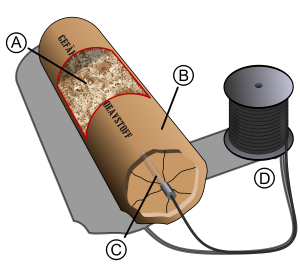
\includegraphics[scale=0.47]{./img/dynamite.png} & 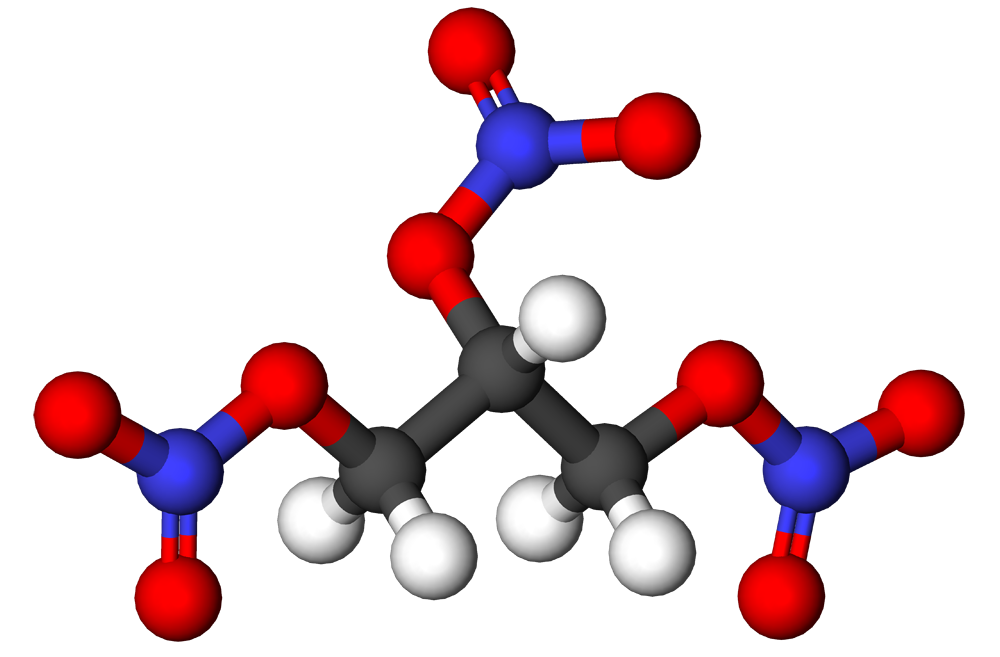
\includegraphics[scale=0.16]{./img/nitroglycerin.png} \\
Dynamite Stick & Nitroglycerin: $C_3 N_3 H_5 O_9$
\end{tabular}
\end{center}

\end{frame}

\section{The Boom}

\begin{frame}{General Uses}
\begin{itemize}
	\item In the Mining Industry,
	\item In Quarrying Industry, especially in marble quarries,
	\item Also Construction Industry and Demolition Industry.
\end{itemize}
\end{frame}

\begin{frame}{Current Uses}
\begin{itemize}
	\item Phrases such as 'It's political dynamite.'.
    \item Songs such as AC\textbackslash DC - T.N.T.
	\item Nowadays blowing up takes places with badass explosives, dynamite
still mainly used in cartoons.
\begin{center}
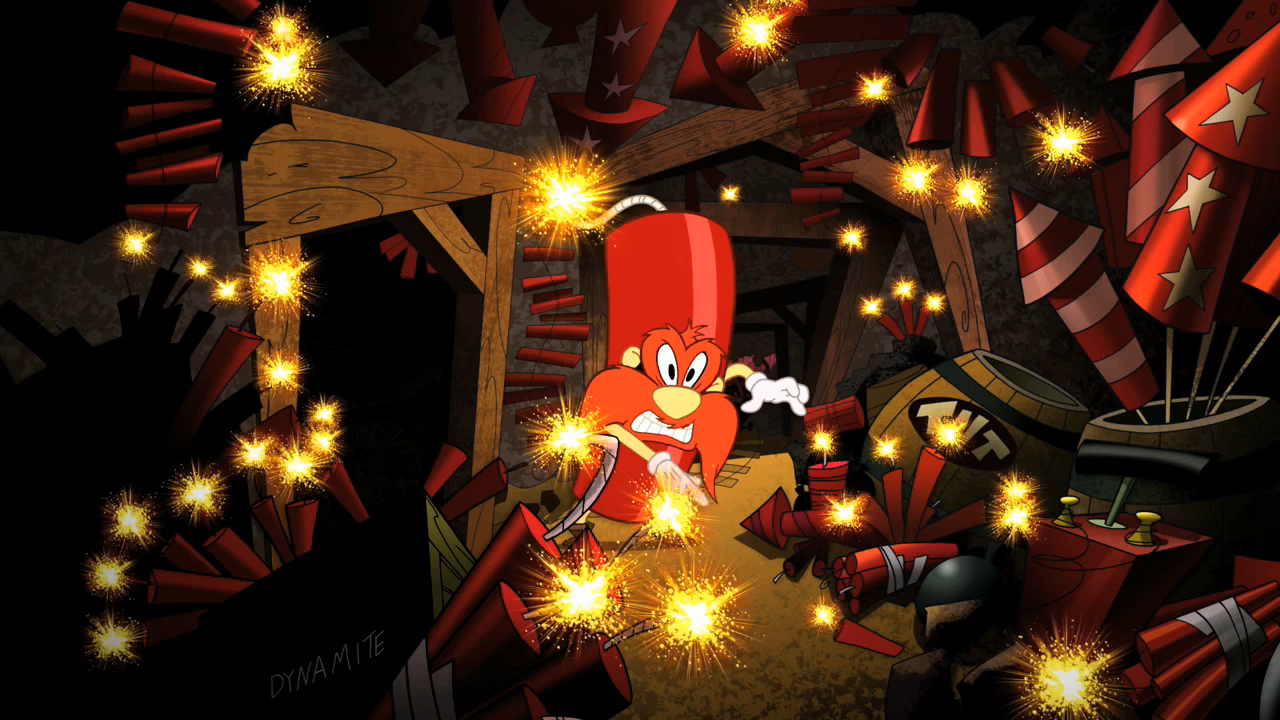
\includegraphics[scale=0.2]{./img/cartoon.png}
\end{center}
\end{itemize}
\end{frame}

\begin{frame}
\begin{center}
\LARGE
Thank you for your undivided attention!

\hbox{}

QUESTIONS?
\end{center}
\end{frame}

\end{document}